\documentclass{amsart}

% I  moved all the document specific preamble stuff here so the top of this document doesn't get messy
\usepackage[english]{babel}
\usepackage{csquotes}
\usepackage[sortcites=true, sorting=nyt, backend=biber]{biblatex}

\usepackage[colorlinks=true,
pdfstartview=FitV, linkcolor=blue, citecolor=olive,
urlcolor=cyan]{hyperref}
\usepackage{xcolor, soul} %Package to insert links, citations, etc.

\usepackage{amsmath, amsthm, amssymb, mathtools}
\usepackage{graphicx} % Required for inserting images
\usepackage{geometry}
\usepackage{multicol}
\usepackage{tabularx}
\usepackage{changepage}
\usepackage[T1]{fontenc}
\usepackage{tikz}
\usepackage{listings} % Used for inserting code snippets
\usepackage{comment}
\usepackage{setspace}
\usepackage{todonotes}
\usepackage{tcolorbox} % used for drawing boxes around paragraphs so that notes are easier to identify

\usepackage{enumitem}
\usepackage{listings} % Used for including code snippets

\geometry{letterpaper, portrait, margin=2in}%1in}

\graphicspath{{Journal_Figures}}

\definecolor{myorange}{HTML}{ff7f00} % Defines the color of the box around text for tcolorbox

%https://osl.ugr.es/CTAN/macros/latex/contrib/tcolorbox/tcolorbox.pdf
\tcbuselibrary{breakable}
\tcbset{%any default parameters
	width=0.7\textwidth,
	halign=justify,
	center,
	breakable,
	colback=myorange    
}

% This controls how the code snippets are typset
\lstset{
	basicstyle=\ttfamily,
	columns=fullflexible,
	frame=single,
	breaklines=true,
	postbreak=\mbox{\textcolor{red}{$\hookrightarrow$}}\space
}

\lstset{language=Octave}


\newtheorem{theorem}{Theorem}[section]
\newtheorem{lemma}[theorem]{Lemma}

\theoremstyle{definition}
\newtheorem{definition}{Definition}[section]
\newtheorem*{example*}{Example}
\newtheorem{example}{Example}


\theoremstyle{remark}
\newtheorem{remark}{Remark}

\newlist{eqlist}{enumerate}{2}
\setlist[eqlist]{label=(\roman*), before=\raggedright}

% Nice way to make notes for myself
\newcommand{\William}[1]{\textcolor{red}{[William] #1}}

% Some nice math macros
\newcommand{\set}[1]{\left\{#1\right\}}
\newcommand*\diff{\mathop{}\!\mathrm{d}} % Changes the font of the differential d when writing dx or similar
\renewcommand{\st}{\colon} % renews the st command that is usually provided by soul to strike through
\newcommand{\N}{\mathbb{N}}
\newcommand{\R}{\mathbb{R}}
\newcommand{\Z}{\mathbb{Z}}
\newcommand{\Q}{\mathbb{Q}}
\newcommand{\RP}{\mathbb{RP}}
\newcommand{\Hyp}{\mathbb{H}}
\newcommand{\T}{\mathcal{T}}

\newcommand{\der}{\mathsf{d}}
\newcommand{\crossratio}[1]{\operatorname{CR}\left[#1\right]}

\newcommand{\metricd}{\operatorname{d}}

% Makes a todo list environment to make nice todo lists for things that would need to be shown
\newlist{todolist}{itemize}{2}
\setlist[todolist]{label=$\square$}

\newcommand{\inquotes}[1]{``#1''}

\newcommand{\close}[1]{\overline{#1}}

\newcommand{\wrt}{\text{w.r.t. }}
\newcommand{\proj}[1]{\pi\left(#1\right)}

\frenchspacing
%\doublespacing

\newenvironment{summary}{
	\hfill \break 
	\begin{center}
		\textbf{Summary:}
	\end{center}
	\begin{adjustwidth}{0.5in}{0.5in}
		
	
}{
\end{adjustwidth}
\bigskip
}

\usetikzlibrary{intersections}

\tikzset{
	convexset/.style = {line width = 0.75 pt, fill = white},
	ext/.style = {circle, inner sep=0pt, minimum size=2pt, fill=black},
	segment/.style = {line width = 0.75 pt}
}





 

% Resource Locations
\graphicspath{{Journal_Figures}}
\bibliography{meeting_journal_references.bib}


\def\WC #1{\footnote{\color{blue} W: #1}}
\def\GM #1{\footnote{\color{magenta} G: #1}}
\def\inn #1{\langle #1\rangle}

\title{Visualizing the Manhattan curve --- Journal}
\author{William Clampitt and Giuseppe Martone}
\date{November 2024}


\begin{document}

\begin{abstract}
    This notebook will serve as a research journal for William's master thesis project.
\end{abstract}

\maketitle
\tableofcontents


\section{November 19, 2024}
\subsection{Meeting notes}
\subsubsection{Counting Problems}
	Gauss estimated that the distribution of prime numbers was 
	\begin{equation*}
		\# \set{p \in P \st p \leq T} \sim \frac{T}{\ln T} 
	\end{equation*}
	
	These type of counting problems are common in fields such as Geometry, Topology, and Dynamical Systems. 
	
	Typically, in this context
	\begin{equation*}
		\# \set{ a \in A \st a \leq T} \sim \text{ exponential in } T
	\end{equation*}
	
	\subsubsection*{Topoligical Entropy}
	Typically, topological entropy is calcualted with the below formula:
	\begin{equation*}
		h_{\text{top}}(A) = \lim_{T \to \infty} \frac{1}{T} \ln \# \set{a \in A \st a \leq T}
	\end{equation*}
	
	\begin{example*}
		\begin{equation*}
			h_{\text{top}}(\N) = 0
		\end{equation*}
	\end{example*}
	
	\subsubsection*{Hilbert Metric First Glance}
	
	\begin{figure}[h]
		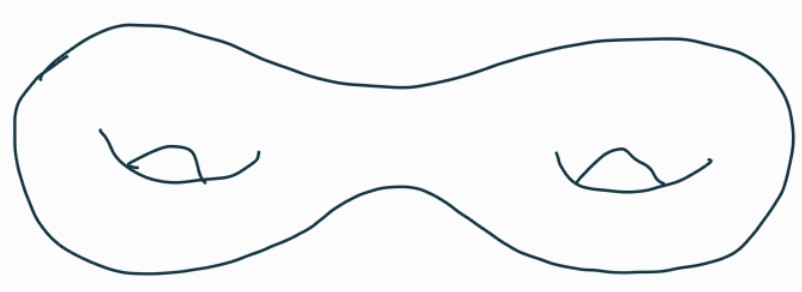
\includegraphics[width=0.5\linewidth]{g2_torus}
		\label{fig:g2_torus}
		\caption{Hyperbolic structure (locally looks like $\mathbb{H}^2$)}
	\end{figure}
	
	\begin{enumerate}
		\item You need a hyperbolic structure on $S$, call it  $p$.
		\item The set of closed loops (discrete)
		\begin{itemize}
			\item Each closed loop has a length \wrt the hyperbolic structure (number $> 0$)
		\end{itemize}
	\end{enumerate}
	
	We will denote the length of the curve $c$ as $l_p(c)$ \wrt $p \in \R$ where $p > 0$.
	\begin{equation*}
		\# \set{c \st l_p(c) < T} \sim \frac{e^T}{T}
	\end{equation*}
	\begin{remark}
		This was shown by Huber Marpulis \William{Is this person the same as Grigory Margulis? Maybe I wrote the name down wrong when I was taking notes.}\GM{Huber proved it for hyperbolic surfaces. G. Margulis generalized it and his proof is more dynamical}
	\end{remark}
	
	\subsubsection*{Origin of Program Matrices}
	
	The three matrices in the first program are representing a relfection accross the three distinct edges of the triangles that are formed when we stretch the holes of our pants to the boundary of our hyperbolic space. 
	
	
\subsection{Post-meeting notes}

\subsubsection{Counting Problems}

\begin{example*}
	The distribution of prime numbers. In 1792 Gauss proposed that
	\begin{equation*}
		\pi(n) \sim \frac{n}{\ln n}
	\end{equation*}
	
	but was later refined to 
	\begin{equation*}
		\pi(n) \sim \text{Li}(n),
	\end{equation*}
	
	where
	\begin{equation*}
		\text{Li}(n) = \int_{2}^{n} \frac{\diff x}{\ln x}
	\end{equation*}\cite{wolfram_prime_num_theorem}
\end{example*}


\section{December 3, 2024}
\subsection{Meeting notes}

\begin{summary}
	In this meeting we discussed the problems that I encountered with my program. In summary, my program is using up too much system memory of the computer. This results in the program crashing which prematurely halts the calculation of the words of our alphabet. Because I was not incrementally storing the already computed matrices, the program would not yeild any results if it crashed. 
\end{summary}



\subsubsection*{Potential Solutions to Problem}
I think one way that might be good to reduce the system memory useage of my program would be to store the words of length $n$ in a file, then use those words to generate the words of length $n + 1$. The words of length $n$ would then be unloaded from system memory. After the words of length $n$ are unloaded, we can use the words of length $n + 1$ to calculated the words of length $n + 2$ and so on. 

\subsection{Post-meeting notes}

I am attempting to rewrite my current program using Octave while also implimenting my idea about iteratively saving the words of length $n$ each time so that I do not have to store the entirety of the list in system memory at one time. After this is done, the list will need to be sifted through to remove duplicates matrices. 

So far it seems like the success of this project would be greatly benifited by reducing the number of matrix multiplications a program would have to do. Currently before any duplicates are removed, generating all of the words up to length $n$ creates $3^{\frac{n(n+1)}{2}}$ matrices. This takes a very long time to compute. My theory though is that this creates a lot of duplicates, especially when we are relitavely close to the origin of our tiling. It would be ideal if we could recognize the conditions that would create a duplicate matrix before having to preform the computation.

From what I understand of what Dr. Martone explained to me in one of our previous meetings is that these matrices represent a reflection across one of the edges of our triangles that are formed by our pairs of pants. I am assuming that the tiling process would begin with a single triangle and then continuously reflect across every edge of each triangle that was formed during this process. 

I am pretty sure that each word we create is representative of a sort of path formed by the reflections about each edge of these triangles. Many of these paths will end up leading to the same place though. \William{I will provide an illustration of my idea here later.} If we could find a more efficient way of tiling the space that minimizes the number of paths that lead to the same place in our tiling, then the computation would hopefully become a lot less resource intensive, which would make it more practical. 

I suspect that this could be done by using some sort of graph to map out triangular grid that is formed by our tiling. We could hopefully calculate the size of our graph by finding the maximum \inquote{radius} that can be reached by words of length $n$, and then using some algorithm to find the shortest amount of reflections that would be required to reach that tile. This would probably be a good place to impliment something like Dijkstra's algorithm which finds the shortest path between nodes in a graph. All of this should be able to be done much more efficiently that just brute forcing thousands of matrix multitplications and then sorting out the duplicates. 

\textbf{TODO List:}
\begin{todolist}
	\item Make sure that I am thinking about these matrices in the right way.
	\item If I am thinking about this the right way, figure out how we could efficiently encode this tiling as a graph. 
	\item I would possibly need to prove that two words that lead to the same triangle actually end up being the same matrix. 
\end{todolist}

\section{December 14, 2024}
\subsection{Meeting Notes}

Dr. Martone seems to think that my graph idea is interesting and it worth looking into further. He was concerned about my graph needing to find the shortest Hilbert distance between nodes; not the shortest number of reflections between nodes. My initial though was that I could weight the edges of he graph in such a way that they mimicked the Hilbert distance. This may still be possible, but it would require more thought to get working properly. 

\subsection{Post-meeting Notes}

I have spent some time working on this program. My first step is to find a way of encoding the graph of words up to a maximum length of $N$ as an adjacency matrix that the computer can work with. I made some observations about the number of triangles that are added to the tiling when going from a max of $N$ words to a max of $N + 1$ words. 

\begin{center}
	\bigskip
	\begin{tabular}{c | c | c}
		length of words & number of nodes added & sum total of nodes\\
		\hline
		$0$ & $1$ & $1$ \\
		$1$ & $3$ & $4$ \\
		$2$ & $6$ & $10$ \\
		$3$ & $9$ & $19$ \\
		$4$ & $12$ & $31$
	\end{tabular}
\end{center}

This can be extrapolated into the formula 
\begin{equation*}
	\text{\# Nodes}(N) = 1 + \sum_{n = 1}^{N} 3n = 1 + \frac{3N (N + 1)}{2}
\end{equation*}

From the work that I have done so far, I think that the most difficult challenge that I am facing right now is encoding the tiling that we have as an adjacency matrix that the computer can work with. Once we have that, there are many implementations of Dijkstra's algorithm that can either be borrowed or modified to fit our needs. I am currently doing some experimentation with algorithms that will generate the adjacency matrix for a graph that represents a tiling of words up to length $N$. 



\section{January 9, 2025}
\section{Meeting Notes}
During this meeting we discussed potential ways of weighting the graph that we worked on last time. After some thinking, Giuseppe thought of an idea to use the cross ratio to find weights for our graph. I have a drawing of the setup we came up with in Figure \ref{fig:graph_weights}.

\begin{figure}[h]
	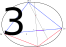
\includegraphics[width=0.75\linewidth]{graph_weighting_cross_ratio}
	\caption{Visualization of method of producing graph weights}
	\label{fig:graph_weights}
\end{figure}

We note that $e_1, e_2, e_3$ are the standard basis vectors in $\R^3$.

\subsection*{The General Case for Distance}

Since $v_2$ is the plane spanned by $v_1$ and $v_4$, $v_2 = a_1 v_1 + a_4 v_4$.

Similarly, since $v_3$ is the plane spanned by $v_1$ and $v_4$, $v_3 = b_1 v_1 + b_4 v_4$.

\begin{figure}[h]
	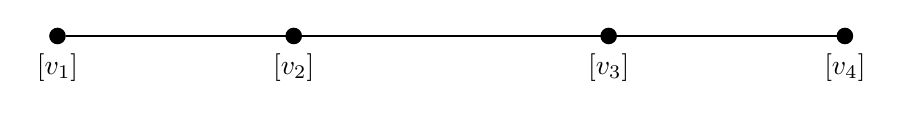
\begin{tikzpicture}[
		dot/.style={circle, fill, minimum size = #1,
			inner sep=0pt, outer sep=0pt},
		dot/.default = 6pt
		]
		\node[dot, label=below:{$[v_1]$}] (v1) at (-5,0) {};
		\node[dot, label=below:{$[v_2]$}] (v2) at (-2,0) {};
		\node[dot, label=below:{$[v_3]$}] (v3) at (2,0) {};
		\node[dot, label=below:{$[v_4]$}] (v4) at (5,0) {};
		
		\draw (v1) -- (v4);
	\end{tikzpicture}
	\caption{General setup for distance.}
	\label{fig:general_distance_setup}
\end{figure}

The distance between $[v_2]$ and $[v_3]$ would be given by
\begin{equation*}
	d([v_2], [v_3]) = \ln \left( \text{Cr}\left[ v_1, v_2, v_3, v_4\right] \right)
\end{equation*}

The cross ratio would be given by
\begin{equation*}
	\text{Cr}\left[ v_1, v_2, v_3, v_4 \right] = \frac{b_4}{a_4} \cdot \frac{a_1}{b_1}
\end{equation*}

\textbf{Claims:}
\begin{itemize}
	\item $\text{Cr}\left[ v_1, v_2, v_3, v_4 \right] > 1$
	\item It doesn't depend on the choice of coordinates. In other words, if we rescale $v_1, v_2, v_3, v_4$ independently, the cross ratio does not change.
	\item For any invertible $3\times3$ matrix $A$, we have $\text{Cr}\left[ Av_1, Av_2, Av_3, Av_4 \right] = \text{Cr}\left[ v_1, v_2, v_3, v_4 \right].$
\end{itemize}

\section{January 14, 2025}
\subsection{Meeting Notes}
I  had some troub

\newpage
\printbibliography

\end{document}
